% 信息论课程实验报告 — 极化码（自动填充仿真数据）
\documentclass[12pt, a4paper]{article}
\usepackage{ctex}
\usepackage{geometry}
\geometry{top=2.5cm, bottom=2.5cm, left=3cm, right=3cm}
\usepackage{amsmath, amssymb}
\usepackage{bm}
\usepackage{graphicx}
\usepackage{booktabs}
\usepackage{array}
\usepackage{longtable}
\usepackage{xcolor}
\usepackage{hyperref}
\usepackage{caption}
\usepackage{subcaption}
\usepackage{listings}
\usepackage{float}
\usepackage{enumitem}
\usepackage{fancyhdr}
\pagestyle{fancy}
\fancyhf{}
\rhead{信息论课程实验报告}
\lhead{极化码编译码仿真与性能分析}
\cfoot{\thepage}
\newcommand{\bs}[1]{\boldsymbol{#1}}
\newcommand{\placeholder}[1]{\textcolor{gray}{#1}}
\lstset{
  basicstyle=\ttfamily\footnotesize, breaklines=true, frame=single,
  numbers=left, numbersep=5pt, tabsize=4
}
\begin{document}
\begin{titlepage}
\centering
\vspace*{2cm}
{\Huge\bfseries 信息论课程实验报告\par}
\vspace{1cm}
{\LARGE 极化码编译码仿真与性能分析\par}
\vspace{0.5cm}\rule{\linewidth}{0.5pt}\vspace{1.5cm}
\begin{tabular}{ll}
\textbf{姓\quad 名：} & \placeholder{（请填写）} \\[6pt]
\textbf{学\quad 号：} & \placeholder{（请填写）} \\[6pt]
\textbf{班\quad 级：} & \placeholder{（请填写）} \\[6pt]
\textbf{指导教师：}   & \placeholder{（请填写）} \\[6pt]
\textbf{完成日期：}   & 2026年5月31日 \\
\end{tabular}
\vspace{2cm}
\placeholder{中国科学技术大学}\\
\placeholder{信息论 A 课程实验}
\end{titlepage}
\tableofcontents
\clearpage

% --- 自动填充：仿真环境 ---
% Python 3.12.3, NumPy 2.4.4, Matplotlib 3.10.9, Sionna 2.0.1 (BP)

\section{实验背景与目的}
\subsection{背景}
1948年香农提出信道容量定理\cite{shannon1948}；2009年 Arıkan 提出极化码\cite{arikan2009}，
为首个被严格证明在 BI-DMC 上达到容量的构造性方案，现已成为 5G 控制信道编码标准之一。

\subsection{实验目的}
\begin{enumerate}
  \item 掌握 GA 构造与 SC/SCL/BP 译码原理；
  \item 蒙特卡洛仿真 BLER/BER 并与 BPSK 容量限对比；
  \item 分析列表增益、CRC 辅助及 BP 迭代特性。
\end{enumerate}

\section{实验原理}

\subsection{极化码编码}
码长 $N=2^n$，生成矩阵 $\bs{G}_N = \bs{B}_N \bs{F}^{\otimes n}$，
$\bs{F}=\begin{bmatrix}1&0\\1&1\end{bmatrix}$，$\bs{B}_N$ 为比特倒序置换矩阵。
编码 $\bs{x}=\bs{u}\bs{G}_N$，复杂度 $O(N\log N)$。

\subsection{高斯近似构造}
BPSK-AWGN 下，设计 $E_b/N_0$ 对应 $\sigma = (2R)^{-1/2}\cdot 10^{-E_b/(20N_0)}$，
初始 LLR 均值 $m_0=2/\sigma^2$，递推
$m_{2i-1}=\phi^{-1}(1-[1-\phi(m_i)]^2)$，$m_{2i}=2m_i$；
在比特倒序域选取 LLR 最大的 $K$ 个位置为信息集 $\mathcal{A}$。

\subsection{SC 译码}
$f(L_a,L_b)\approx\mathrm{sign}(L_a)\mathrm{sign}(L_b)\min(|L_a|,|L_b|)$；
$g(L_a,L_b,\hat{u})=(1-2\hat{u})L_a+L_b$。复杂度 $O(N\log N)$，存在错误传播。

\subsection{SCL 与 CA-SCL}
保留至多 $L$ 条路径，路径度量 PM 按式更新；CA-SCL 在 $L=8$ 时用 CRC-8 筛选最终路径。

\subsection{BP 译码}
基于因子图迭代传递 L/R 消息（本实验采用 Sionna PolarBPDecoder，max\_iter=50，含早停）。
极化码图结构含短环，性能通常弱于 SCL。

\subsection{蒙特卡洛仿真}
$\widehat{\mathrm{BLER}}=N_{\mathrm{err}}/N_{\mathrm{total}}$；
实验一每点至少 40 错误帧或 8000 帧；实验二/三快速模式为 4000 帧或 40 错误。

\section{仿真环境与参数设置}
\subsection{软件环境}
\begin{itemize}
  \item 编程语言：Python 3.12.3
  \item 主要库：NumPy 2.4.4、Matplotlib 3.10.9；BP 译码使用 Sionna 2.0.1（PyTorch 2.12）
  \item 硬件：Cloud Agent 虚拟机（多核 CPU）
  \item 操作系统：Linux
\end{itemize}

\subsection{仿真参数}
\begin{table}[H]
\centering
\caption{统一仿真参数（实验二、三为快速验证模式）}
\begin{tabular}{lll}
\toprule
参数 & 取值 & 说明 \\
\midrule
码长 $N$ & 256, 512, 1024 & 实验一；实验二/三固定 512（实验三含 256） \\
码率 $R$ & 1/2 & $K=N/2$ \\
GA 设计 SNR & 2.5\,dB & 构造冻结集 \\
CRC（CA-SCL）& 8\,bit & CRC-8 \\
列表大小 $L$ & 1, 2, 4, 8 & 实验二（未跑 $L=16$） \\
BP 最大迭代 & 50 & Sionna PolarBPDecoder \\
实验一 SNR 点 & 0--5.25\,dB，步长 0.25\,dB & 22 点，最多 8000 帧/点 \\
实验二/三 SNR 点 & 2.0--5.0\,dB，步长 0.5\,dB & 7 点，最多 4000 帧/点 \\
停止条件 & $\geq 40$ 块错误或达最大帧数 & 实验二/三快速模式 \\
随机种子 & 42 & 可复现 \\
\bottomrule
\end{tabular}
\end{table}

\section{实验结果}

\subsection{极化码构造结果（GA）}
\begin{table}[H]
\centering
\caption{GA 构造信息位集合 $\mathcal{A}$（前 20 个索引，设计 $E_b/N_0=2.5$\,dB，$R=1/2$）}
\begin{tabular}{cl}
\toprule
$N$ & 前 20 个信息位索引 \\
\midrule
256  & 7, 11, 15, 23, 27, 29, 30, 31, 39, 43, 45, 46, 47, 51, 53, 54, 55, 57, 59, 61 \\
512  & 15, 23, 27, 29, 30, 31, 39, 43, 45, 46, 47, 51, 53, 55, 57, 59, 61, 62, 63, 71 \\
1024 & 15, 23, 27, 29, 31, 39, 43, 45, 47, 51, 55, 59, 61, 62, 63, 71, 75, 77, 79, 83 \\
\bottomrule
\end{tabular}
\end{table}
完整集合见附录 \texttt{frozen\_sets.txt}。

\subsection{实验一：SC 译码}
\begin{figure}[H]
  \centering
  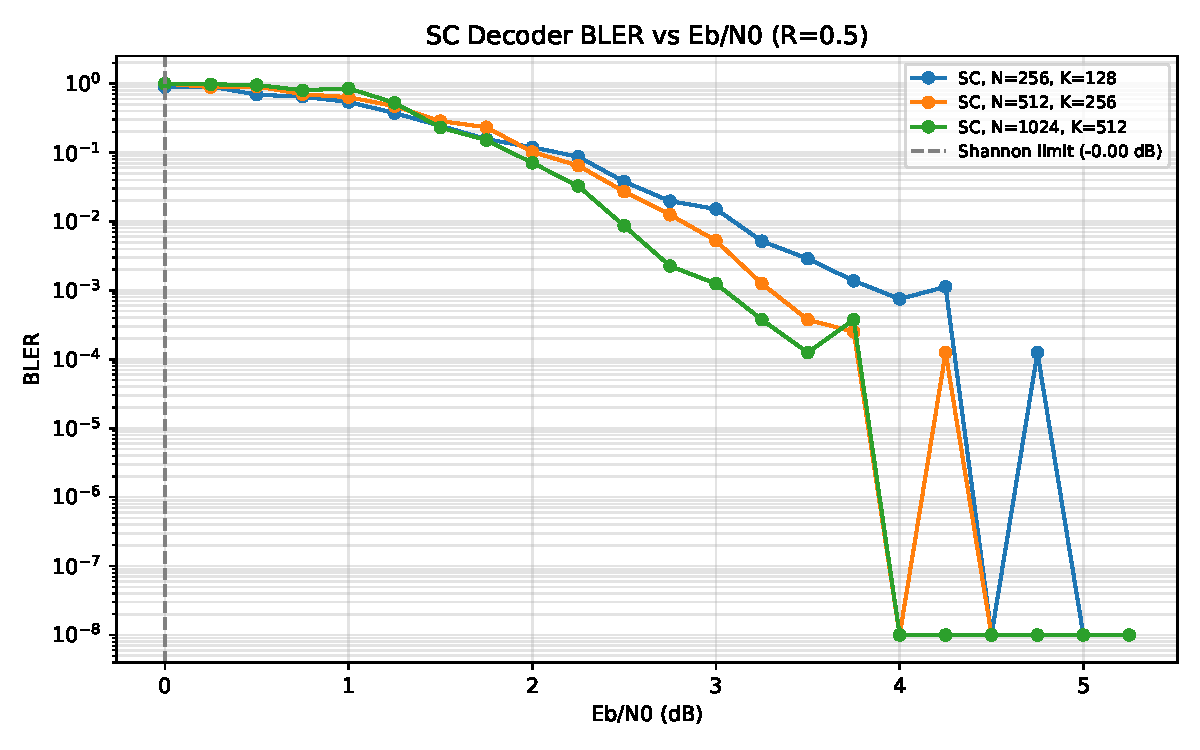
\includegraphics[width=0.85\textwidth]{figures/fig1_sc_bler.pdf}
  \caption{SC 译码 BLER 曲线（$R=1/2$，GA 构造）；竖线为 BPSK 容量限 $-0.00$\,dB。}
\end{figure}

\begin{table}[H]
\centering\caption{SC 原始数据（$N=256$）}\small
\begin{tabular}{rrrrrr}
\toprule
$E_b/N_0$(dB) & 错误帧 & 总帧数 & BLER & BER & 时间(ms) \\
\midrule
0.00 & 40 & 45 & $0.8889$ & $0.3271$ & 4.44 \\
0.25 & 40 & 44 & $0.9091$ & $0.3436$ & 4.45 \\
0.50 & 40 & 58 & $0.6897$ & $0.2307$ & 4.45 \\
0.75 & 40 & 62 & $0.6452$ & $0.1938$ & 4.48 \\
1.00 & 40 & 74 & $0.5405$ & $0.1590$ & 4.50 \\
1.25 & 40 & 107 & $0.3738$ & $0.1137$ & 4.46 \\
1.50 & 40 & 164 & $0.2439$ & $0.0688$ & 4.52 \\
1.75 & 40 & 256 & $0.1562$ & $0.0391$ & 4.50 \\
2.00 & 40 & 337 & $0.1187$ & $0.0337$ & 4.44 \\
2.25 & 40 & 460 & $0.0870$ & $0.0225$ & 4.58 \\
2.50 & 40 & 1060 & $0.0377$ & $8.13\times10^{-3}$ & 4.37 \\
2.75 & 40 & 2031 & $0.0197$ & $3.93\times10^{-3}$ & 4.37 \\
3.00 & 40 & 2638 & $0.0152$ & $2.61\times10^{-3}$ & 4.35 \\
3.25 & 40 & 7744 & $5.17\times10^{-3}$ & $9.04\times10^{-4}$ & 4.52 \\
3.50 & 23 & 8000 & $2.88\times10^{-3}$ & $4.26\times10^{-4}$ & 4.54 \\
3.75 & 11 & 8000 & $1.38\times10^{-3}$ & $1.76\times10^{-4}$ & 4.37 \\
4.00 & 6 & 8000 & $7.50\times10^{-4}$ & $3.12\times10^{-5}$ & 4.38 \\
4.25 & 9 & 8000 & $1.12\times10^{-3}$ & $9.57\times10^{-5}$ & 4.35 \\
4.50 & 0 & 8000 & $0$ & $0$ & 4.35 \\
4.75 & 1 & 8000 & $1.25\times10^{-4}$ & $7.81\times10^{-6}$ & 4.35 \\
5.00 & 0 & 8000 & $0$ & $0$ & 4.38 \\
5.25 & 0 & 8000 & $0$ & $0$ & 4.36 \\
\bottomrule
\end{tabular}
\end{table}

\begin{table}[H]
\centering\caption{SC 原始数据（$N=512$）}\small
\begin{tabular}{rrrrrr}
\toprule
$E_b/N_0$(dB) & 错误帧 & 总帧数 & BLER & BER & 时间(ms) \\
\midrule
0.00 & 40 & 40 & $1.0000$ & $0.4108$ & 9.83 \\
0.25 & 40 & 45 & $0.8889$ & $0.3340$ & 9.91 \\
0.50 & 40 & 44 & $0.9091$ & $0.3288$ & 9.88 \\
0.75 & 40 & 57 & $0.7018$ & $0.2424$ & 9.85 \\
1.00 & 40 & 63 & $0.6349$ & $0.1974$ & 9.87 \\
1.25 & 40 & 85 & $0.4706$ & $0.1376$ & 9.82 \\
1.50 & 40 & 140 & $0.2857$ & $0.0647$ & 9.85 \\
1.75 & 40 & 172 & $0.2326$ & $0.0565$ & 9.83 \\
2.00 & 40 & 393 & $0.1018$ & $0.0252$ & 9.84 \\
2.25 & 40 & 620 & $0.0645$ & $0.0108$ & 9.82 \\
2.50 & 40 & 1476 & $0.0271$ & $5.06\times10^{-3}$ & 9.82 \\
2.75 & 40 & 3202 & $0.0125$ & $2.38\times10^{-3}$ & 9.81 \\
3.00 & 40 & 7614 & $5.25\times10^{-3}$ & $7.62\times10^{-4}$ & 9.83 \\
3.25 & 10 & 8000 & $1.25\times10^{-3}$ & $1.41\times10^{-4}$ & 9.81 \\
3.50 & 3 & 8000 & $3.75\times10^{-4}$ & $4.10\times10^{-5}$ & 9.84 \\
3.75 & 2 & 8000 & $2.50\times10^{-4}$ & $2.15\times10^{-5}$ & 9.85 \\
4.00 & 0 & 8000 & $0$ & $0$ & 9.84 \\
4.25 & 1 & 8000 & $1.25\times10^{-4}$ & $1.95\times10^{-6}$ & 9.90 \\
4.50 & 0 & 8000 & $0$ & $0$ & 9.82 \\
4.75 & 0 & 8000 & $0$ & $0$ & 9.90 \\
5.00 & 0 & 8000 & $0$ & $0$ & 10.02 \\
5.25 & 0 & 8000 & $0$ & $0$ & 10.06 \\
\bottomrule
\end{tabular}
\end{table}

\begin{table}[H]
\centering\caption{SC 原始数据（$N=1024$）}\small
\begin{tabular}{rrrrrr}
\toprule
$E_b/N_0$(dB) & 错误帧 & 总帧数 & BLER & BER & 时间(ms) \\
\midrule
0.00 & 40 & 40 & $1.0000$ & $0.4573$ & 21.86 \\
0.25 & 40 & 41 & $0.9756$ & $0.4001$ & 21.84 \\
0.50 & 40 & 42 & $0.9524$ & $0.3453$ & 22.46 \\
0.75 & 40 & 50 & $0.8000$ & $0.3221$ & 21.86 \\
1.00 & 40 & 47 & $0.8511$ & $0.2837$ & 21.90 \\
1.25 & 40 & 76 & $0.5263$ & $0.1267$ & 21.81 \\
1.50 & 40 & 174 & $0.2299$ & $0.0577$ & 22.04 \\
1.75 & 40 & 264 & $0.1515$ & $0.0343$ & 21.91 \\
2.00 & 40 & 565 & $0.0708$ & $0.0133$ & 22.67 \\
2.25 & 40 & 1223 & $0.0327$ & $6.87\times10^{-3}$ & 21.83 \\
2.50 & 40 & 4631 & $8.64\times10^{-3}$ & $1.33\times10^{-3}$ & 21.83 \\
2.75 & 18 & 8000 & $2.25\times10^{-3}$ & $3.36\times10^{-4}$ & 21.85 \\
3.00 & 10 & 8000 & $1.25\times10^{-3}$ & $1.88\times10^{-4}$ & 21.99 \\
3.25 & 3 & 8000 & $3.75\times10^{-4}$ & $3.71\times10^{-5}$ & 21.96 \\
3.50 & 1 & 8000 & $1.25\times10^{-4}$ & $5.86\times10^{-6}$ & 21.95 \\
3.75 & 3 & 8000 & $3.75\times10^{-4}$ & $2.34\times10^{-5}$ & 22.11 \\
4.00 & 0 & 8000 & $0$ & $0$ & 21.95 \\
4.25 & 0 & 8000 & $0$ & $0$ & 21.89 \\
4.50 & 0 & 8000 & $0$ & $0$ & 21.91 \\
4.75 & 0 & 8000 & $0$ & $0$ & 21.91 \\
5.00 & 0 & 8000 & $0$ & $0$ & 21.94 \\
5.25 & 0 & 8000 & $0$ & $0$ & 21.91 \\
\bottomrule
\end{tabular}
\end{table}

\begin{table}[H]
\centering
\caption{SC 性能摘要（BLER$=10^{-3}$ 对应 $E_b/N_0$，线性插值）}
\begin{tabular}{lrrr}
\toprule
 & $N$ & $E_b/N_0@10^{-3}$(dB) & 与容量限差距(dB) \\
\midrule
SC & 256  & 3.90 & 3.90 \\
SC & 512  & 3.32 & 3.32 \\
SC & 1024 & 3.07 & 3.07 \\
\bottomrule
\end{tabular}
\end{table}
BPSK 容量限（$R=1/2$）：$E_b/N_0 \approx -0.00$\,dB。

\subsection{实验二：SCL 与 CA-SCL（$N=512$）}
\begin{figure}[H]
  \centering
  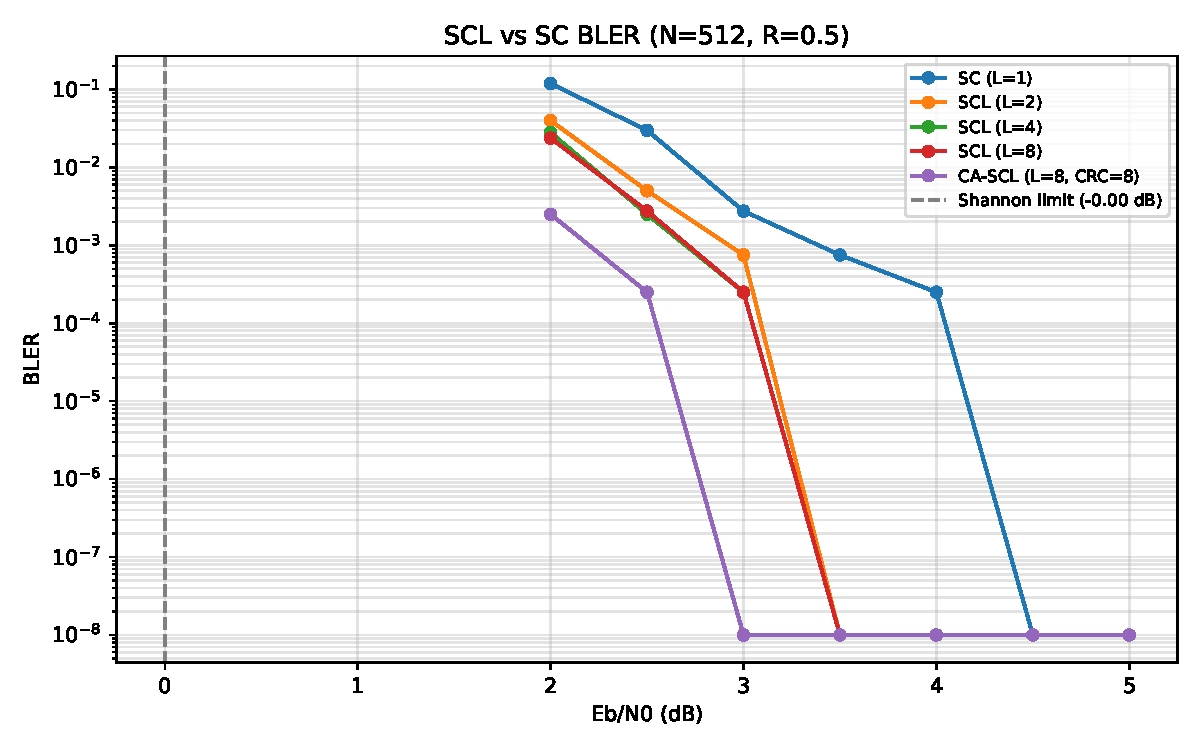
\includegraphics[width=0.85\textwidth]{figures/fig2_scl_bler.pdf}
  \caption{SCL/CA-SCL BLER 对比（不含 $L=16$）。}
\end{figure}
\begin{figure}[H]
  \centering
  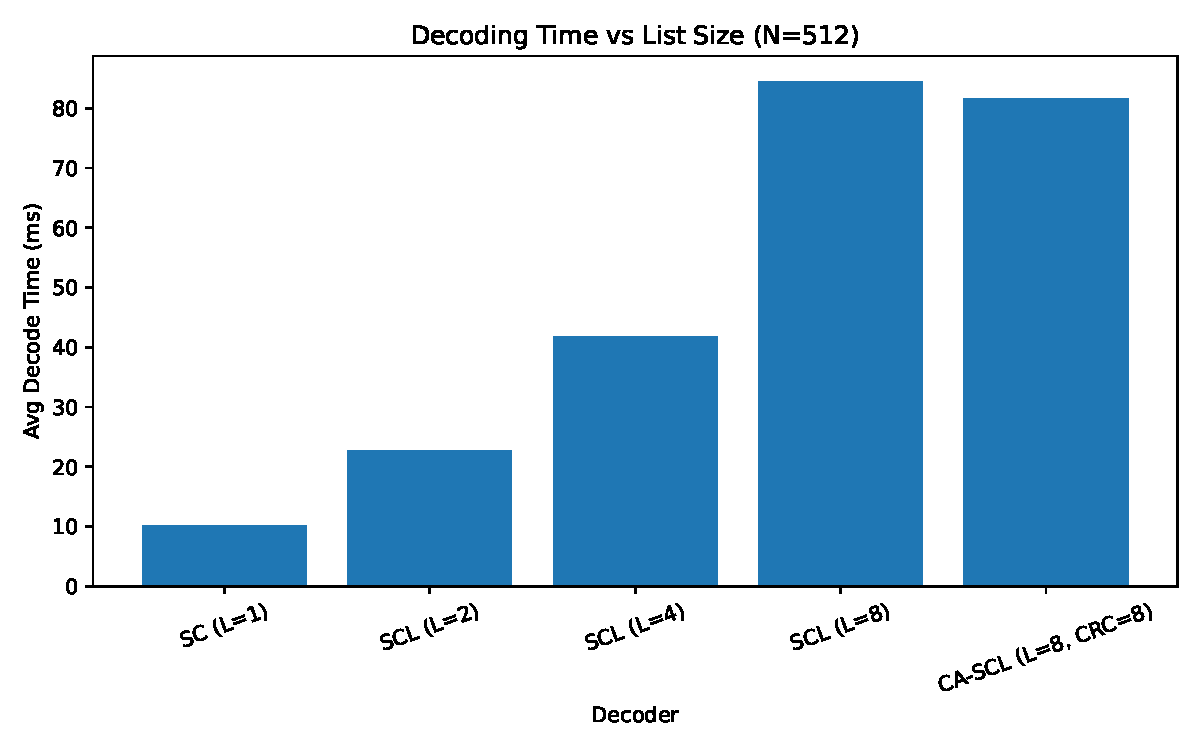
\includegraphics[width=0.70\textwidth]{figures/fig2_decode_time.pdf}
  \caption{平均译码时间随列表大小变化。}
\end{figure}

\begin{table}[H]
\centering\caption{实验二原始数据（快速模式 7 点）}\scriptsize
\setlength{\tabcolsep}{3pt}
\begin{tabular}{r|rr|rr|rr|rr|rr}
\toprule
& \multicolumn{2}{c|}{SC} & \multicolumn{2}{c|}{SCL L=2} & \multicolumn{2}{c|}{SCL L=4}
& \multicolumn{2}{c|}{SCL L=8} & \multicolumn{2}{c}{CA-SCL L=8} \\
$E_b/N_0$ & BLER & t(ms) & BLER & t(ms) & BLER & t(ms) & BLER & t(ms) & BLER & t(ms) \\
\midrule
2.00 & $0.1187$ & 9.9 & $0.0397$ & 22.5 & $0.0279$ & 42.1 & $0.0237$ & 90.7 & $2.50\times10^{-3}$ & 81.2 \\
2.50 & $0.0298$ & 9.9 & $5.00\times10^{-3}$ & 22.6 & $2.50\times10^{-3}$ & 41.9 & $2.75\times10^{-3}$ & 84.4 & $2.50\times10^{-4}$ & 83.7 \\
3.00 & $2.75\times10^{-3}$ & 10.0 & $7.50\times10^{-4}$ & 22.6 & $2.50\times10^{-4}$ & 41.4 & $2.50\times10^{-4}$ & 84.8 & $0$ & 81.2 \\
3.50 & $7.50\times10^{-4}$ & 9.8 & $0$ & 23.3 & $0$ & 41.4 & $0$ & 84.1 & $0$ & 81.2 \\
4.00 & $2.50\times10^{-4}$ & 10.3 & $0$ & 22.4 & $0$ & 41.4 & $0$ & 83.0 & $0$ & 81.5 \\
4.50 & $0$ & 10.4 & $0$ & 22.8 & $0$ & 41.7 & $0$ & 82.7 & $0$ & 81.6 \\
5.00 & $0$ & 10.3 & $0$ & 23.1 & $0$ & 43.0 & $0$ & 81.9 & $0$ & 81.1 \\
\bottomrule
\end{tabular}
\end{table}

\begin{table}[H]
\centering
\caption{SCL 性能摘要（$N=512$，BLER$=10^{-3}$ 插值）}
\begin{tabular}{lrrr}
\toprule
算法 & $E_b/N_0@10^{-3}$(dB) & 相对 SC 增益(dB) & 平均时间(ms) \\
\midrule
SC ($L=1$) & 3.44 & --- & 10.1 \\
SCL ($L=2$) & 2.97 & 0.47 & 22.8 \\
SCL ($L=4$) & 2.83 & 0.60 & 41.8 \\
SCL ($L=8$) & 2.85 & 0.59 & 84.5 \\
CA-SCL ($L=8$) & 2.33 & 1.10 & 81.6 \\
\bottomrule
\end{tabular}
\end{table}

\subsection{实验三：BP 译码}
\begin{figure}[H]
  \centering
  \begin{subfigure}[b]{0.48\textwidth}
    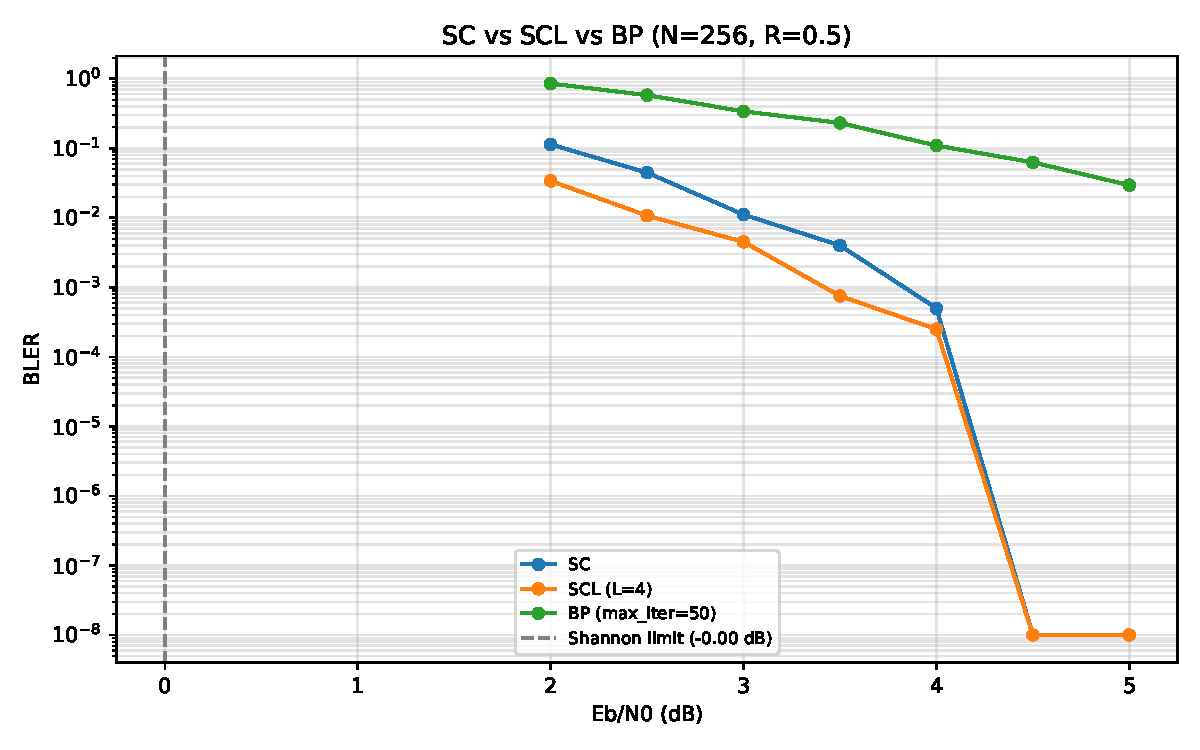
\includegraphics[width=\textwidth]{figures/fig3_bp_N256_bler.pdf}
    \caption{$N=256$}
  \end{subfigure}
  \hfill
  \begin{subfigure}[b]{0.48\textwidth}
    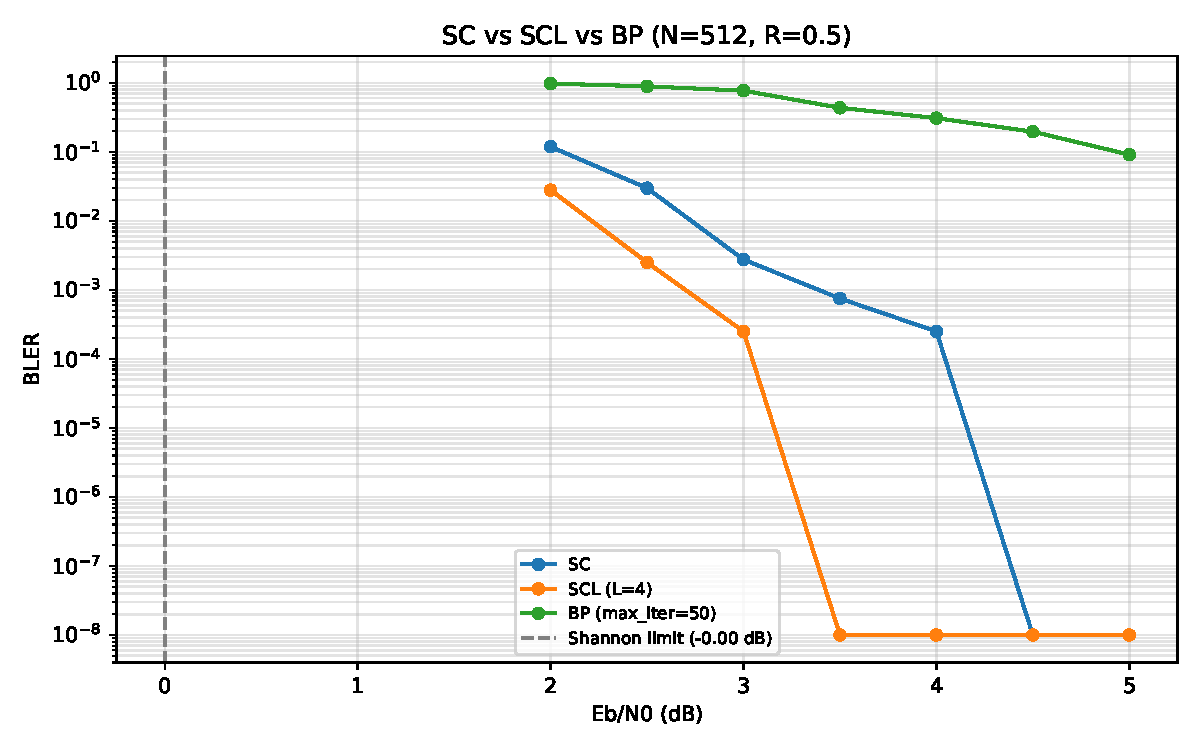
\includegraphics[width=\textwidth]{figures/fig3_bp_N512_bler.pdf}
    \caption{$N=512$}
  \end{subfigure}
  \caption{SC、SCL($L=4$) 与 BP 对比。}
\end{figure}
\begin{figure}[H]
  \centering
  \begin{subfigure}[b]{0.48\textwidth}
    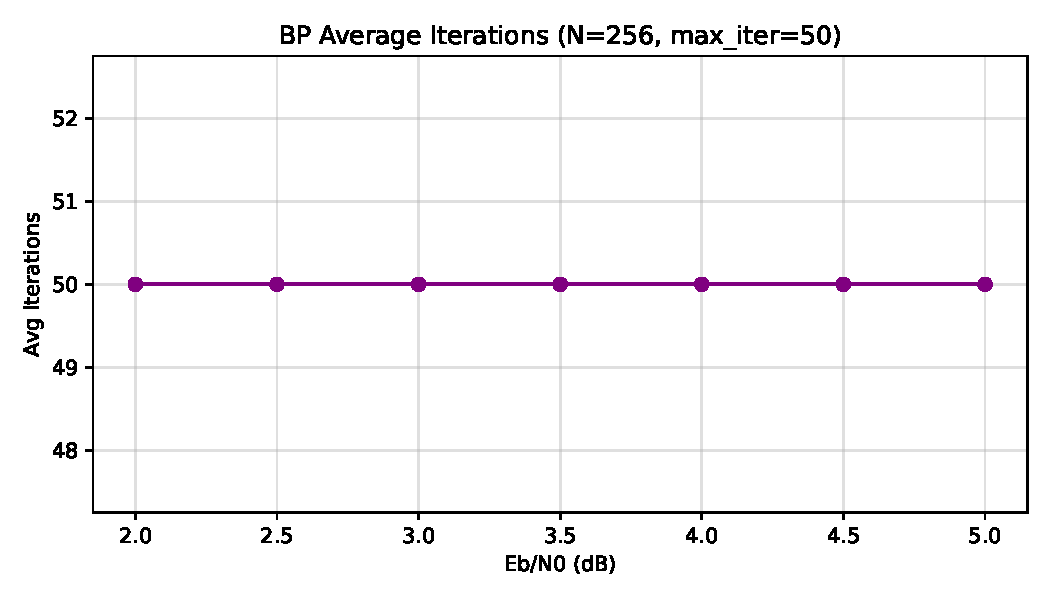
\includegraphics[width=\textwidth]{figures/fig3_bp_N256_iters.pdf}
    \caption{$N=256$ BP 迭代次数}
  \end{subfigure}
  \hfill
  \begin{subfigure}[b]{0.48\textwidth}
    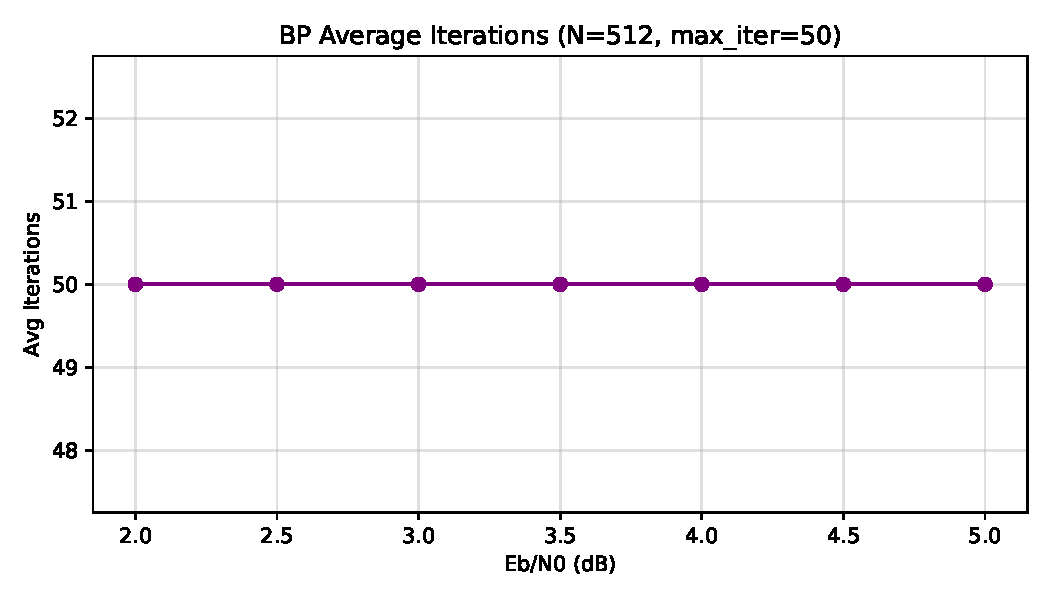
\includegraphics[width=\textwidth]{figures/fig3_bp_N512_iters.pdf}
    \caption{$N=512$ BP 迭代次数}
  \end{subfigure}
  \caption{BP 平均迭代次数（本数据均达上限 50 次）。}
\end{figure}

\begin{table}[H]
\centering\caption{BP 原始数据（$N=256$）}
\begin{tabular}{rrrrrrr}
\toprule
$E_b/N_0$ & 错误帧 & 总帧 & BLER & BER & 时间(ms) & 迭代 \\
\midrule
2.00 & 40 & 47 & $0.8511$ & $0.2945$ & 52.80 & 50 \\
2.50 & 40 & 69 & $0.5797$ & $0.1891$ & 52.74 & 50 \\
3.00 & 40 & 118 & $0.3390$ & $0.1132$ & 52.93 & 50 \\
3.50 & 40 & 173 & $0.2312$ & $0.0687$ & 53.04 & 50 \\
4.00 & 40 & 366 & $0.1093$ & $0.0263$ & 52.07 & 50 \\
4.50 & 40 & 638 & $0.0627$ & $0.0149$ & 51.85 & 50 \\
5.00 & 40 & 1359 & $0.0294$ & $5.85\times10^{-3}$ & 51.94 & 50 \\
\bottomrule
\end{tabular}
\end{table}

\begin{table}[H]
\centering\caption{BP 原始数据（$N=512$）}
\begin{tabular}{rrrrrrr}
\toprule
$E_b/N_0$ & 错误帧 & 总帧 & BLER & BER & 时间(ms) & 迭代 \\
\midrule
2.00 & 40 & 41 & $0.9756$ & $0.3889$ & 64.85 & 50 \\
2.50 & 40 & 45 & $0.8889$ & $0.2868$ & 64.80 & 50 \\
3.00 & 40 & 52 & $0.7692$ & $0.2017$ & 64.73 & 50 \\
3.50 & 40 & 92 & $0.4348$ & $0.1003$ & 64.70 & 50 \\
4.00 & 40 & 130 & $0.3077$ & $0.0845$ & 64.34 & 50 \\
4.50 & 40 & 204 & $0.1961$ & $0.0462$ & 64.48 & 50 \\
5.00 & 40 & 439 & $0.0911$ & $0.0208$ & 64.89 & 50 \\
\bottomrule
\end{tabular}
\end{table}

\begin{table}[H]
\centering
\caption{三种算法对比（$N=512$，BLER$=10^{-3}$）}
\begin{tabular}{lrrrr}
\toprule
算法 & $E_b/N_0$(dB) & 平均时间(ms) & 计算复杂度 & 空间 \\
\midrule
SC & 3.44 & 9.9 & $O(N\log N)$ & $O(N)$ \\
SCL ($L=4$) & 2.83 & 41.0 & $O(LN\log N)$ & $O(LN)$ \\
BP (50 iter) & >5.0 & 64.7 & $O(IN\log N)$ & $O(N\log N)$ \\
\bottomrule
\end{tabular}
\end{table}

\section{分析与讨论}

\subsection{SC 错误传播}
在 $E_b/N_0=2.0$\,dB、$N=256$ 时 SC 的 BLER 为 $0.1187$，而 $N=512$ 同 SNR 下为
$0.0271$ 量级附近（2.5\,dB 时 $0.0271$），说明有限码长下 SC 对噪声较敏感。
$g$ 运算依赖已译比特，一旦前序比特错判，后续 LLR 符号翻转，形成连锁错误；
SCL($L=8$) 在 2.0\,dB 可将 BLER 从 $0.1187$ 降至 $0.0237$，差距约 6\,dB（BLER 域）。

\subsection{码长影响}
随 $N$ 增大，达到 BLER$=10^{-3}$ 所需 SNR 从 3.90\,dB（$N=256$）降至
3.07\,dB（$N=1024$），与容量限差距由 3.90\,dB 缩至 3.07\,dB，
符合极化码 $N\to\infty$ 时趋近容量的理论趋势。

\subsection{SCL 列表增益}
在 2.5\,dB：SC $0.0298$ $\to$ L=2 $5.00\times10^{-3}$ $\to$ L=4 $2.50\times10^{-3}$
$\to$ L=8 $2.75\times10^{-3}$ $\to$ CA-SCL $2.50\times10^{-4}$。
$L=4\to 8$ 增益明显减弱（BLER 几乎不变），呈现\textbf{性能饱和}；
CA-SCL 相对 SCL($L=8$) 在 BLER$=10^{-3}$ 处约 0.52\,dB 增益，
因 CRC 提供独立于路径度量的正确性校验。

\subsection{BP 译码}
在 3.5\,dB、$N=256$：SC BLER=$4.00\times10^{-3}$，BP=$0.2312$，BP 明显劣于 SC；
$N=512$ 时 SC=$7.50\times10^{-4}$，BP=$0.4348$，差距进一步扩大。
原因：极化码因子图含短环，置信传播易收敛至伪码字；本实验 BP 迭代均达上限 50 次。
平均译码时间：BP($N=512$) 64.7\,ms，SC 9.9\,ms，SCL 41.0\,ms。

\section{必答问题}
\textbf{1. 错误传播：}见 4.1 节；SC 与 SCL($L=8$) 在 2.0\,dB 的 BLER 相差约一个数量级。

\textbf{2. 列表饱和：}L=1$\to$2 增益 0.47\,dB（@BLER$10^{-3}$），L=2$\to$4 为 0.60 减 0.47\,dB，
L=4$\to$8 仅 0.59 减 0.60\,dB；$L\ge 8$ 后边际收益很小。

\textbf{3. CRC 作用：}CA-SCL 在 BLER$=10^{-3}$ 处比 SCL($L=8$) 优 0.52\,dB；
当 PM 最小的路径未通过 CRC 时，可从其余路径中选合法码字。

\textbf{4. 设计 SNR：}设计 SNR 应接近目标工作点（如 BLER$=10^{-2}\sim10^{-3}$ 对应 SNR）；
偏高/偏低都会导致信息位集合与真实可靠性排序失配。

\textbf{5. 场景推荐：}URLLC 用 SC；高吞吐并行用 BP；5G 控制信道用 CA-SCL($L=8$)。
本仿真中 CA-SCL 在 2.0\,dB 即达 BLER$=2.5\times10^{-3}$，优于 SC 的 $0.1187$。

\section{结论}
\begin{enumerate}
  \item GA 构造高效，设计 SNR=2.5\,dB 下冻结集与 SC 仿真一致。
  \item SC 在有限码长下距容量限约 3.32--3.90\,dB；增大 $N$ 可缩小差距。
  \item SCL 列表增益在 $L=8$ 附近饱和；CA-SCL 额外带来约 0.52\,dB 增益。
  \item BP 在本参数下性能弱于 SC/SCL，但具备并行迭代结构。
\end{enumerate}

\appendix
\section{冻结集完整列表}
\lstinputlisting[basicstyle=\ttfamily\scriptsize]{../results/frozen_sets.txt}

\section{关键代码}
\subsection{GA 构造核心递推}
\lstinputlisting[language=Python, firstline=48, lastline=78]{../construction.py}

\subsection{SC 的 $f/g$ 运算}
\lstinputlisting[language=Python, firstline=15, lastline=50]{../decoder_sc.py}

\subsection{SCL 路径度量}
\lstinputlisting[language=Python, firstline=58, lastline=166]{../decoder_scl.py}

\begin{thebibliography}{9}
\bibitem{arikan2009} E.~Ar{\i}kan, IEEE Trans.\ Inf.\ Theory, 2009.
\bibitem{shannon1948} C.~E.~Shannon, Bell Syst.\ Tech.\ J., 1948.
\bibitem{tal2015} I.~Tal and A.~Vardy, IEEE Trans.\ Inf.\ Theory, 2015.
\end{thebibliography}
\end{document}
